\chapter{Problèmes difficiles en théorie des nombres}
    \section{Complexité et cryptographie}
        \subsection{Introduction}
            Idée : mesurer la "difficulté" algorithmique d'un problème.
            \begin{defi} (Problème de décision)
                Un problème de décision est une collection d'instances qui sont des ensembles de données qui admettent exactement une des deux réponses "oui" ou "non".
            \end{defi}
            \begin{expl}
                \begin{enumerate}
                    \item Problème SAT (Satisfaisabilité) 
                    \begin{description}
                        \item[Instance :] Une fonction à variables booléenne $F : \{0,1\}^n \to \{0, 1\}$ construite avec les connecteurs logiques $\lor, \land, \lnot$. Par exemple,
                        \begin{align*}
                            f(x_1, x_2, x_3, x_4) = (\lnot (x_1 \land (\lnot x_3))) \lor (x_1 \land x_2 \land (\lnot x_1))
                        \end{align*}
                        \item[Question :] existe-t-il $x_1, \cdots, x_n \in \{0, 1\}$ temls que $F(x_1, \cdots, x_n) = 1$ ?
                        \item[Algorithme :] recherche exhaustive sur $(x_1, \cdots, x_n)$, la complexité est en $\mathcal{O}(2^n)$.
                    \end{description}
                    \item FBQ (Formes Booléennes Quantifiées)
                    \begin{description}
                        \item[Instance :] Une formule booléenne avec quantificateur e.g. $\forall x_i \exists x_j \cdots F(x_1, \cdots, x_n)$ ($F$ est une fonction booléenne comme dans SAT)
                        \item[Question :] Cette formule est-elle vraie ? 
                        \item[Algorithme :] Recherche exhaustive ($\mathcal{O}(2^n)$).  
                    \end{description}
                    \item Equations diophantiennes ($10^\text{ème}$ problème de Hilbert)
                    \begin{description}
                        \item[Instance :] Une équation polynomiale à plusieurs inconnues et à coefficients entiers
                        \item[Question :] Cette équation admet-elle des solutions entières ?
                        \item[Algorithme :] Matyasevich, 1971 : il n'y a pas d'algo qui répond à cette question.  
                    \end{description}
                \end{enumerate}
            \end{expl}

        \subsection{Calculabilité au sens de Turing}
            Turing : Cryptanalyse d'Enigma, construction de machines dédiées à la cryptanalyse d'Enigma, Machine de Turing.
            
            \subsubsection{Modèle de Turing}
                On dispose d'un ruban infini
                \begin{figure}[H]
                    \centering
                    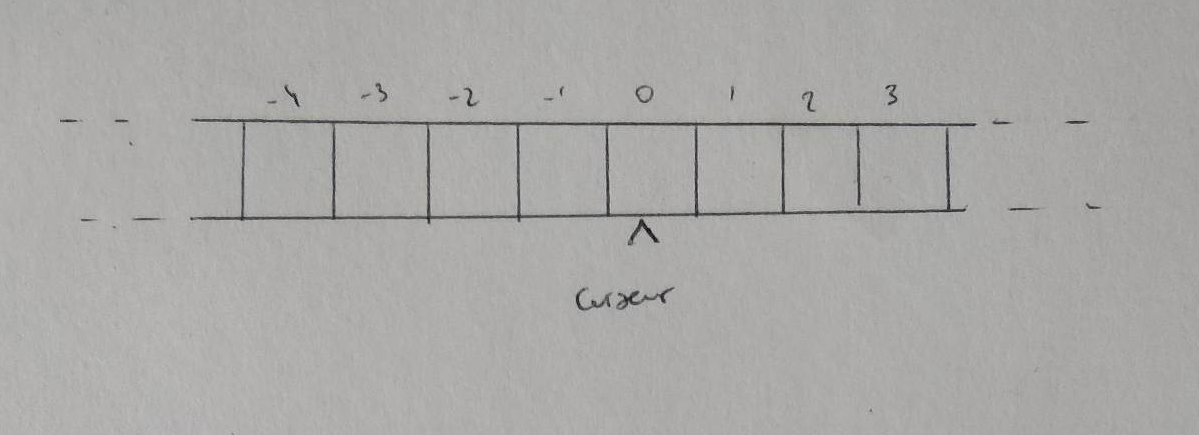
\includegraphics[width=.5\textwidth]{01}
                \end{figure}
                Chaque case contient un symbôle (dans un alphabet fini $\Sigma$ que l'on peut supposer être $\{0, 1\}$, ou le symbôle blanc $b$). Le ruban v aêtre lu case par case par le curseur, la machine est à chaque instant dans un état $q_i \in Q$, où $Q$ est l'ensemble fini des états possibles.
                \begin{defi} (Machine de Turing)
                    Une opération élémentaire est entièrement déterminée par le symbôle lu par le curseur, et par l'état actuel $q_i$ :
                    \begin{enumerate}
                        \item Le curseur remplace le symbôle par un élément de $\Sigma \cup \{b\}$
                        \item Le curseur de déplae soit d'une case vers la gauche, soit d'une case vers la droiten, soit reste sur place.
                        \item La machine passe de l'état $q_i$ à l'état $q_j$.
                    \end{enumerate}
                    Une machine de Turing est donc la donnée d'une fonction
                    \begin{align*}
                        M : (\Sigma \cup \{b\}) \times Q \to (\Sigma \cup \{b\}) \times \{-1, 0, 1\} \times Q
                    \end{align*}
                \end{defi}
                \begin{defi} (Calcul déterministe)
                    Le calcul déterministe d'une entrée $x$ avec une machine de Turing $M$ est la suite d'opération suivante :
                    \begin{enumerate}
                        \item La machine est commence par être dans l'état $q_0$
                        \item Le curseur est placé sur la case $1$
                        \item $x$ est écrite sur les cases $1, \cdots, n$ du ruban, les autres contenant $b$.
                        \item On applique itérativement $M$, le calcul se terine lorsque la machine atteint l'état final $q_F$. La sortie $y$ est alors la donnée inscrite sur le ruban lorsque la machine termine.
                    \end{enumerate}
                \end{defi}
                Terminologie : L'ensemble des suites finies de symbôles de $\Sigma$ est noté $\Sigma^*$. Un mot est un élément de $\Sigma^*$. Une fonction $f : \Sigma^* \to \Sigma^*$ est turing calculable s'il existe une machine de Turing $M$ qui sur tout entrée $x \in \Sigma^*$ calcule $y = f(x)$.

        \subsection{Complexités en temps et classes $P$, $NP$}
            \begin{defi}
                La longeuru d'un calcul sur une entrée $x \in \Sigma^*$ pour une machine de Turing $M$ est le nombre $t_M(x)$ d'opération élémentaires qui composent le calcul. Ainsi on défini la complexité en temps d'une machine de Turing comme
                \begin{align*}
                    \begin{array}{cccc}
                        T_M : & \mathbb{N} & \to & \mathbb{N} \\
                        & n & \mapsto & \max_{\substack{x \in \Sigma^* \\ |x| = n}} \{t_M(x)\} \\
                    \end{array}
                \end{align*}
            \end{defi}
            \begin{defi}
                Un algorithme polynomial $\mathcal{A}$ pour calculer $f$ est une machine de Turing $M$ qui calcule $f$ et telle qu'il existe un polynôme $p$ tel que $\forall n \in \mathbb{N}$, $T_M(n) \leq p(n)$. On appelle classe $P$ l'ensemble des problèmes de décision admettant un algorithme polynomial.
            \end{defi}
            \begin{defi}
                On dit qu'un pb de décision est calculable par un algo non déterministe polynomial s'il existe une machien de Turing $M$ et un polynome $p$ tel que 
                \begin{enumerate}
                    \item La réponse est oui pour l'entrée $x$ ssi il existe $y \in \Sigma^*$ (certificat) tel que $M$ calcule $1$ lorsqu'on met $x \in \Sigma^*$ dans les cases $1$ à $n$ et $y$ dans les cases $-1$ a $-m$.
                    \item Pour tout $x$ donnant la réponse $1$, $M$ calcule $1$ et temps $\leq p(n)$
                \end{enumerate}
                On appelle classe $NP$ la classe des problèmes de décision admettant un algorithme non déterministe polynomial.
            \end{defi}
            \begin{remq}
                $P \subseteq NP$.
            \end{remq}
            
        \subsection{Problèmes $NP$-complets}
            \begin{defi}
                On dit que le problème de décision $p_1$ se réduit au problème de décision $p_2$ s'il existe une fonction $\varphi : \Sigma^* \to \Sigma^*$ calculable en temps polynomial telle que la réponse à $p_1$ est oui pour l'entrée $x$ si et seulement si la réponse à $p_2$ est oui pour l'entrée $\varphi(x)$.
            \end{defi}
            \begin{nota}
                On note $p_1 \ltimes p_2$.
            \end{nota}
            \begin{prop}
                $p_1 \in P$ et $p_1\ltimes p_2 \Rightarrow p_1 \in P$
            \end{prop}
            \begin{defi}
                Un problème $\Pi$ est $NP$-complet ssi $\forall p \in NP$, $p \ltimes \Pi$.
            \end{defi}
            \begin{theo} (Cook, 1971)
                SAT est $NP$-complet.
            \end{theo}
            \begin{remq}
                Si $SAT \ltimes P$, alors $P$ est $NP$-complet.
            \end{remq}
            \begin{expl}
                \begin{enumerate}
                    \item SAT
                    \item $3$-SAT
                    \item Circuit hamiltonien
                    \item $3$-coloriabilité d'un graphe
                    \item TSP
                    \item Pb du sac à dos
                    \item Système de $n$ équations quadratiques sur un $\mathbb{F}_2$.
                \end{enumerate}
            \end{expl}
            On conjecture que $P \neq NP$. Astuce de Levin : Supposons que $P = NP$ : alors on peut construire un algorithme polynomial pour résoudre $SAT$. Considérons les machines de Turing $M_1, M_2, \cdots$ qui prennent en entrée une instance de $SAT$ : Alors on fait tourner les machines simultanément, en faisant tourner de une étape $M_1$, puis en faisant tourner de une étape $M_2$, puis $M_1$, puis $M_3$, $M_2$ et $M_1$, etc. 

            \subsubsection{Résumé de la hiérarchie des complexités algorithmiques :}
                \begin{figure}[H]
                    \centering
                    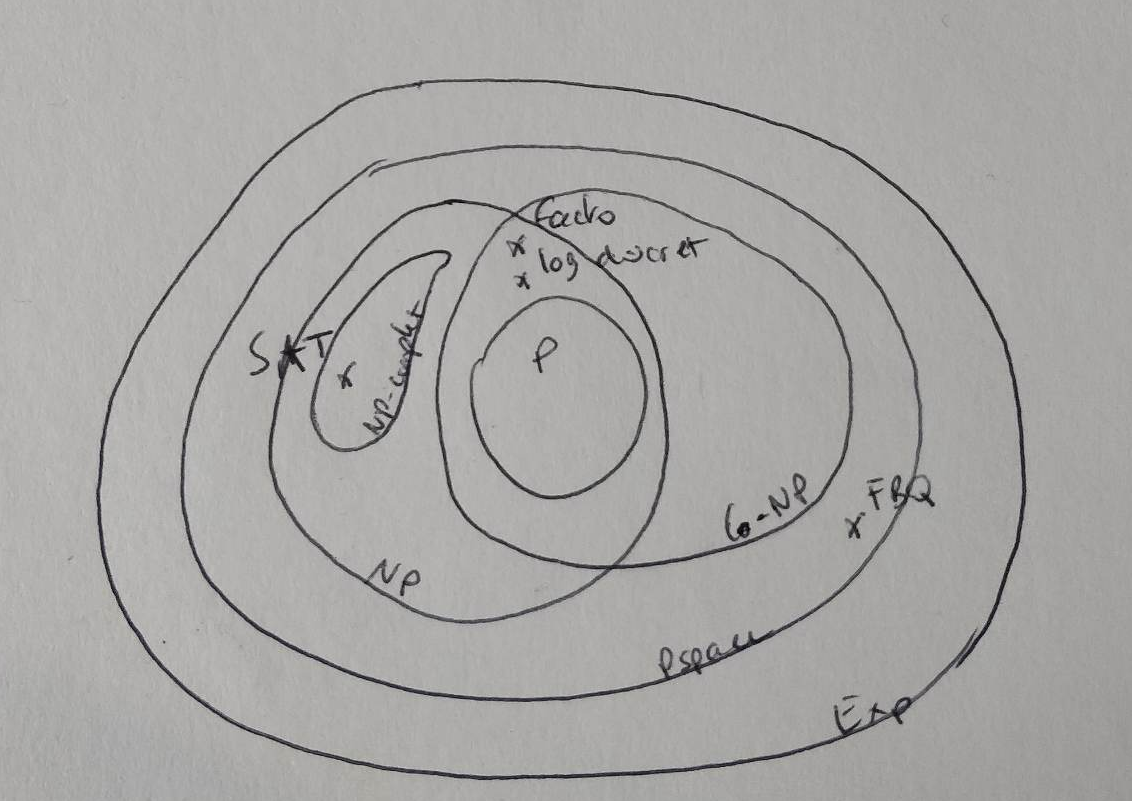
\includegraphics[width=.5\textwidth]{02}
                \end{figure}
                \begin{remq}
                    Co-$NP \cap NP$-complet $= \emptyset$.
                \end{remq}

    \section{Factorisation}
        \subsection{Complexité}
            Problème de décision FACTM (problème des facteurs majorés)
            \begin{itemize}
                \item Instance : $n$ entier, $M \leq n$.
                \item Question : Existe-t-iil un diviseur de $n$ qui est $\leq M$.
            \end{itemize}
            Si on a un algo polynomial de factorisation, alors on peut résoudre FACTM en temps polynomial. Inversement, Supposons $\mathcal{A}$ algo polynomial pour FACTM. Comment factoriser $n$ ? Soit $p$ le plus petit facteur premier de $n$, alors
            \begin{itemize}
                \item On applique $\mathcal{A}(n, \sqrt{n})$. Si l'algorithme répond non, alors on termine et on répond non (car $n$ est alors premier)
                \item Sinon, on applique $\mathcal{A}(n, \sqrt{n}/2)$. Si l'algo répond non, alors $p \in [\sqrt{n}/2, \sqrt{n}]$, et sinon $p \in [1, \sqrt{n}/2]$.
                \item On continue la dichotomie jusqu'à ce que la taille de l'intervalle obtenu soit plus petite que $1$.
            \end{itemize}
            L'algorithme termine dès que $\sqrt{n}/2^k <1$, où $k$ est le nombre d'appels de $\mathcal{A}$. Ainsi il y a $k = \log_2(\sqrt{n})$ est donc de l'ordre de $\log n$. Une fois $p$ trouvé, on recommence l'algo avec $n/p$. On va recommencer le nombre de facteurs premiers de $n$ (comptés avec leur multiplicité). Mais
            \begin{align*}
                n = \prod_i p_i^{\alpha_i} \geq \prod_i 2^{\alpha_i} = 2^{\sum \alpha_i}
            \end{align*}
            donc $\sum \alpha_i < \log_2 n$, et c'est aussi le nombre de facteurs premiers de $n$ (comptés avec leur multiplicité). Au total, l'algorithme est polynomial.

        \subsection{Idée de Fermat}
            \begin{itemize}
                \item L'idée naïve est d'essayer de diviser par les entiers successifs $\leq n$. C'est en $\mathcal{O}(n)$ donc exponentiel en la taille de l'entier.
                \item On peut aussi s'arrêter avant $\sqrt{n}$, mais l'algorithme reste exponentiel.
                \item On peut aussi diviser par les nombres premiers $\sqrt{n}$. D'après le théorème des nombres premiers (Hadamard, de la Vallée-Poussin), le cardinal des entiers premiers plus petits que $x$ est aymptotiquement équivalent à $x/\ln x$. Ainsi l'algo est en $\mathcal{O}(\sqrt{n}/\log n)$, qui reste exponentiel en la taille de $n$.
            \end{itemize}
            
            